\chapter{Physics of accreting black holes}
\Glspl{BH} are believed to emit no radiation on their own (except, perhaps, hypothetical Hawking radiation, see \citealt{Hawking1974}). 
However, black holes manifest themselves through interaction with other bodies, matter, and radiation in a number of ways.
These include, for instance, light bending, accretion, ejection (in form of relativistic jets and accretion winds), and gravitational waves.
Thus, if a black hole is found in a vicinity of another astrophysical object, it will manifest itself in some way, altering the behaviour and evolution of its neighbours.

Black holes are naturally subdivided into several groups, namely supermassive black holes found in the centres of galaxies (with masses up to $5\times10^{10}~M_\odot$, see \citealt{Shemmer2004, Mehrgan2019}), and stellar-mass black holes, remnants of bright and massive stars, which reached the end of their lifecycle.
The existence of the third group was confirmed by recent discoveries of \gls{BH}-\gls{BH} mergers, which formed \glspl{BH} as massive as $\sim 150~M_\odot$ \citep{Abbott2020}.

Stellar mass black holes are usually formed as a result of a collapse of a massive star.
When the core is no longer capable of sustaining nuclear burning, and further compacting does not increase pressure, so hydrostatic equilibrium is no longer preserved, the star implodes, leaving a naked core, which, depending on its mass, can collapse to a black hole \citep{Woosley2002}.
The core collapse is a complicated process and its outcome depends on the properties of the dying star.
It is possible that the final explosion disrupts the core, leaving no remnant \citep{Kasen2011}, or that the core collapses into a black hole while the outer layers of the star are still intact, which results in a violent act of accretion.

A black hole is formed as a result of a collapse of a singular star if the remnant mass exceeds critical value, known as Tolman-Oppenheimer-Volkoff limit \citep{Tolman1939,Oppenheimer1939,Oppenheimer1939a}.
The largest neutron stars observed so far have masses reaching $\sim 2.2~M_\odot$ \citep{Cromartie2020}, which is below the theoretically predicted limit.
Stellar mass black holes are observed to have masses larger than $\sim 5~M_\odot$ \citep{Ozel2010}, and $[3;~5]~M_\odot$ interval is the lower mass gap \citep{Farr2011, Kreidberg2012}.
An upper limit is believed to be $40 - 65~M_\odot$, set in practice by the (pulsational) pair instability supernovae producing remnants with lower masses than expected in the absence of this instability, or no remnants at all \citep{Woosley2017, Woosley2019}.
More massive objects fall into the upper mas gap (yet a \gls{BH}-\gls{BH} merger \GWxix\ is believed to have at least one of its \gls{BH} components within the gap, see \citealt{LIGOVIRGO2020}).

These limits, however, apply to the process of a collapse of a single star.
If instead, two black holes are formed in a binary system, orbit of which shrinks with time owing to the gravitational wave emission, resulting in a \gls{BH}-\gls{BH} merger, then the result of this merger can have larger mass limited only by the initial masses of the colliding black holes.
\GWxix\ is an example of such merger, producing a $\sim 150~M_\odot$ black hole, which falls in the second mass gap \citep{Abbott2020}.

Galactic black holes are found in binary systems, where they (much like other compact objects) reveal themselves through the interaction with their companion stars.
Such unique configuration -- a degenerate \textit{primary} star and a main sequence (or evolved) \textit{secondary} star -- is, however, hard to achieve, as a system has to survive collapse of a progenitor of the primary star, which can potentially disrupt the binary. 
Another plausible scenario is gravitational capture, when an existing binary star comes in close contact with a remnant of another star, forming a new binary with a compact object, leaving one of the initial stars single.
The probability of formation of a binary system hosting a compact object is relatively low (a few per cent of core-collapse supernovae produce systems with interacting \gls{BH}, \citealt{Kochanek2019}), thus, even though the majority of stars in the Galaxy are believed to be part of binary systems \citep[][$\sim 50\%$ of solar-type stars, see e.g.]{Tian2018}, the binaries with compact objects constitute a tiny fraction of all population \citep[][of the order of hundreds of \glspl{LMXB} in the Milky Way]{Shao2020}, and even smaller number of such systems can be observed and reliably identified.


\section{Accretion onto compact objects in binary systems}
Accreting binary systems hosting compact objects are known to be powerful X-ray sources.
This is attributed to the fact that the accretion process itself is highly efficient in transforming matter into energy compared to, e.g., nuclear fusion that powers non-degenerate stars.
The relationship between the amount of energy $E$ emitted in all wavelengths per unit of time and the amount of matter $M$ consumed within the same time interval can be expressed as follows \citep{AccretionPower}:
\begin{equation}
    \frac{\dd E}{\dd t} = \eta \frac{\dd M}{\dd t} c^2,
\end{equation}
where $c$ is speed of light and $\eta$ is efficiency of the process.
The value of accretion efficiency is usually assumed to be $\sim 0.1$, but can approach $\sim 0.4$ for extreme Kerr black holes \citep{Thorne1974}, which is several orders of magnitude larger than that of hydrogen burning ($\eta_\mrm{nuc} \approx 7 \times 10^{-3}$, \citealt{AccretionPower}).

X-ray binaries can be subdivided into two categories based on their binary mass ratio $q = M_2 / M_1$, where $M_1$ and $M_2$ are masses of primary (accreting) and secondary (donor) stars, respectively.
Low-mass X-ray binaries tend to have main-sequence to giant stars of late spectral type with masses $ \le 1~M_\odot$ as their donors, while high-mass X-ray binaries contain early-type bright massive stars.
The distributions of these systems in the Galactic coordinates reflect the distribution of Population I/II stars: \glspl{HMXB} are found in the Galactic plane, while \glspl{LMXB} are observed closer to the bulge and in globular clusters \citep{Casares2017}.

The spectral types and masses of the donor stars affect the geometry of the accretion processes undergoing in the \glspl{XRB}.
\glspl{LMXB} are powered by the accretion through the Lagrange $L_1$ point if the donor star fills its Roche lobe (Roche lobe overflow).
Despite typically small radius of donor stars, this becomes possible because of a small binary mass ratio, which affects the characteristic size $R_2^\mrm{Roche}$ of secondary star Roche lobe \citep{Eggleton1983, Paczynski1983}:
\begin{equation}
    R_2^\mrm{Roche} \approx 0.46 a \left(\frac{q}{1 + q}\right)^{1/3},
\end{equation}
where $a$ is major semi-axis.

When donor star approaches the equipotential surface, it becomes distorted, and its outer layers can flow through the $L_1$ into the Roche lobe of accretor.
From the perspective of an accretor, the infalling matter has a substantial angular momentum owing to the orbital motion of the system.
This prevents matter from falling directly onto the primary; instead, the continuous gas stream follows an elliptical orbit around the primary.
The process can continue until the stream intersects itself, completing a full rotation around the central body, which is imminent because all particles that enter the Roche lobe through the $L_1$ have angular momentum predominantly in the orbital plane.
The characteristic radius, at which the infalling matter form the ring-like structure, is the circularization radius, which depends on the binary mass ratio $q$ \citep{Plavec1964, AccretionPower}:
\begin{equation}
    R_\mrm{circ} = a (1 + q)\left(0.500 - 0.227 \log q\right)^4.
\end{equation}


The stream of matter, however, cannot stay in an elliptical orbit configuration.
There are several physical processes occurring on different time scales that govern the evolution of this unstable structure.
First, the interaction between different layers of the circling stream leads to internal heating and energy dissipation via radiation on the time scale $t_\mrm{rad}$.
Second, Keplerian differential rotation allows for angular momentum transport in radial direction owing to the shear viscosity, but on a much larger time scale $t_\mrm{visc}$.
With orbital time scale $t_\mrm{orb}$, the following inequality holds true \citep{AccretionPower}:
\begin{equation}
    t_\mrm{orb} < t_\mrm{rad} < t_\mrm{visc}.
\end{equation}
This effectively means that the stream of matter dissipates energy while orbiting the accretor, occupying the most energy-efficient orbit -- circular.
The matter then slowly redistributes angular momentum in radial direction, removing it from the inner edge of the ring and adding at the outer edge.
As a result, the inner edge moves closer to the accreting object, while the outer moves in the opposite direction, expanding the ring to form a geometrically thin accretion disc \citep{Shakura1973, Novikov1973}.
Thus accretion disc allows for an efficient way of stripping excessive angular momentum from the infalling matter, lowering it toward accretor.


A completely different picture is observed in \glspl{HMXB}.
With $q > 1$, it is much harder for the donor star to overflow its Roche lobe.
Still, the components of a \gls{HMXB} are able to exchange mass via a different mechanism.
A hot and massive early-type donor star produces violent stellar winds at a rate of up to $10^{-5}~M_\odot~\mrm{yr}^{-1}$ \citep{AccretionPower}, which is being swept by the compact object in orbit around the donor.
The radius, within which a compact object can capture and, eventually, accrete matter, is determined by the accretor mass and its speed relative to the stellar wind (which is usually highly supersonic).
As a result, accretion happens within a narrow region around the accretor, allowing for the formation of the accretion disc.


\section{Accretion disc in \glsentryplural{LMXB}}
The accretion process of \gls{LMXB} gives rise to a variety of physical phenomena (apart from thin disc), which produce radiation in different energy ranges.
Understanding the complex interplay between these components and their observed manifestations can shed more light on the accretion-ejection mechanism in the vicinity of compact objects -- especially when these compact objects are black holes.

Owing to the simplicity of black holes, their lack of hard surfaces, the accretion process is determined mainly by the following parameters: black hole mass, black hole spin, and mass accretion rate (scaled to Eddington luminosity, see e.g. \citealt{Done2007}).
The process of accretion is also regulated by the binary mass ratio, which has a natural upper limit of $\sim 5/6$ \citep{AccretionPower}, arising from the fact that mass exchange leads to changes in geometrical properties of a system, including the secondary star Roche lobe.
For a system with $q > 5/6$ the flow of matter from donor's lobe into the accretor's is thus accelerating until the ratio falls below the critical value (and any angular momentum loss boosts the redistribution process).
In systems with $q < 5/6$ changes in binary mass ratio result in expansion of donor's lobe, allowing secondary star to evolve and expand.


However, the thin disc solution described in \citet{Shakura1973} is unstable at low accretion rates.
Being optically thick, disc is susceptible to changes in temperatures around hydrogen ionization limit ($\sim 6500$~K, \citealt{Mineshige1993}).
The disc can build up via steady accretion from the donor, until the ionization process starts at some radii.
The process is self-sustaining and spreads both inward and outward, ionizing the whole disc \citep{Lasota2001, Dubus2001}.
The second, viscous, instability is triggered by the rapid increase in temperature, which results in increase of the accretion rate.
At a given radius, more mass is transferred toward inner radii than received from the outer annuli, which eventually decreases pressure and temperature.
This triggers the reverse hydrogen ionization instability, effectively cooling the disc and returning it to the state with conditions close to initial.


A simple theoretical view of the standard thin disc suggests that \glspl{LMXB} are transient objects -- they are likely to remain in a quiescent (i.e. non-active) state for long periods of time and undergo periods of activity and increased brightness -- so-called outbursts.
The instability mechanism responsible for the outbursts allows theses systems to experience multiple periods of activity within short periods of time, effectively making at least some of the \glspl{LMXB} recurrent.
The difference between outburst and quiescence is expected to be drastic as the hydrogen ionization instability produces rather sharp changes in local opacity and, as a result, observed properties of \glspl{LMXB}.



\section{Observed properties of \glsentryplural{BHXRB}}
To date, dozens of systems that fit the description of \gls{BHXRB} have been observed.
A new galactic source is reported, on average, every year.
Attempts are made to maintain lists of black hole X-ray binary candidates and confirmed \glspl{BHXRB}.
This includes, e.g., catalogues like the \gls{WATCHDOG} and \gls{BlackCAT}.

Even though \glspl{LMXB} are studied extensively, it is still challenging to determine the mass of the compact object -- a key parameter that allows for separation black hole from neutron star binaries.
Several dozens of sources have been dynamically confirmed to host an object small and massive enough to be called a black hole.
Other binaries remain candidates.

The first evidence suggesting the existence of black hole binaries came with the beginning of the X-ray era and with discovery of Cyg~X-1  \citep{Bolton1972,Webster1972}, a persistent source.
\iA, the first transient X-ray source, was discovered later \citep{Elvis1975}.
Observations of transients revealed that these object show complex spectral evolution and variability profiles \citep{HBMB05,McClintock2006,Remillard2006,Belloni2010}.

During an outburst a transient can be found in one of the distinct spectral states, which can be identified using X-ray spectral and timing properties.
Observed spectra can be loosely categorized, based on the hardness ratio (the ratio of flux in high-energy X-ray band to low-energy band, e.g. $F_{10-20~\mrm{keV}} / F_{2-6~\mrm{keV}}$, \citealt{Tananbaum1972}), as `hard' state, which is  present during initial and final phases and demonstrates non-thermal spectra, `soft' thermal-dominant state, which is typically observed in the middle phase of the outburst, and transitions between these states. 
A notable example of transient \glspl{LMXB} that do not follow this pattern is \GRSxix\ \citep{Belloni2000}, which spectral states cannot be easily classified as `hard' or `soft'.
The time intervals, over which \glspl{BHXRB} undergo outbursts, differ significantly.
In general, the amount of time a \gls{LMXB} spends in an outburst is smaller than (or, for some objects like \SwiftJxvii, comparable to) that spent in quiescence \citep{Tetarenko2016}. 
This is not true for \gls{HMXB}, which are persistent sources.

There are many more quiescent \glspl{BHXRB} than those seen in outburst \citep{Shao2020}.
The duration of quiescent periods can exceed the duration of the X-ray astronomy era, which for some objects allows only one detection of an X-ray outburst throughout the history of observations.


\section{Multi-component view of the \glsentryplural{BHXRB}}
The observed radiation of \glspl{BHXRB} can originate from one or more of the following components: accretion disc, hot accretion flow, and relativistic jet \citep[see][]{Poutanen2014a,Uttley2014}.
Emission of each component can be scattered by other media, including winds, which further modifies the observed spectrum.
It is worth mentioning that the hot spot, at which the infalling matter intersects the already established accretion disc, can be a prominent source of variable emission in the quiescence (\citealt{Smak1970,Lyutyi1973}, but also \citealt{Bisikalo1998}).
In some cases (like low-luminosity quiescence), emission from the donor star becomes important (see \citealt{Charles2006}, also \citet{Chevalier1989} and \citet{Heida2017} for direct estimates of secondary emission fraction).
The contribution of the donor star can be further boosted if the accreting black hole produces enough X-rays to irradiate one of the sides of the donor, locally increasing the temperature of its outer layers.



\subsection{Spectral properties}
An outburst of a \gls{LMXB} starts at low luminosity with hard power-law X-ray spectrum having cutoff below $\sim 100~\mrm{keV}$ \citep{Belloni2011}.
The luminosity increases substantially with little to no changes to the hardness ratio, followed up by a rapid transition to the soft state at nearly constant luminosity, which results in a dramatic change of the X-ray spectral shape, resembling that of a black body with temperature close to $\sim~1\mrm{keV}$ and a non-thermal tail \citep{Zdziarski2004a, McClintock2006, Done2007}.
The soft-state luminosity drops slowly, usually following an exponential profile \citep{Lasota2001}.
At some point a reverse transition happens, again, with a nearly constant (but much lower than that of the hard-to-soft transition) bolometric luminosity, and the observed X-ray spectrum becomes once again non-thermal.
From this hard state, a transient decays to the quiescent level.
Owing to the difference between transition luminosities, a transient system traces a characteristic hysteresis-like \textit{q}-shaped pattern on the hardness-intensity diagram, which observed shape, however, depends on the inclination angle at which the system is viewed \citep{MunozDarias2013}.


A different picture is seen in radio.
\gls{BHXRB} transients are observed to exhibit prominent power-law ($F \propto \nu^\alpha$, where $\alpha$ is the spectral slope) radio spectra.
The slope is usually variable, and can change on the timescale of hours \citep[e.g.,][]{Gandhi2011}.
A universal correlation between radio and X-ray luminosities found to hold true for the majority of black hole transients (see, e.g., \citealt{Gallo2003, Merloni2003, Corbel2013, Gallo2014}) suggests a shared mechanism responsible for emission in both energy ranges.
Radio component disappears in the soft state \citep{Russell2011a}, and re-emerges with the reverse transition \citep[e.g.,][]{Corbel2000}, in some cases accompanied by relativistic polar outflows large enough to be resolved by modern radio telescopes \citep[e.g., ][]{Bright2020}.
Such optically thin outflows are sometimes observed during state transitions \citep{Kalemci2013}.


The spectral energy distribution is even more complicated in the \gls{ONIR} region.
Blackbody-like spectra are observed in the soft state, while in the hard state \gls{ONIR} flares are usually present, displaying a much harder spectrum \citep{Jain2001}.
An excess over the blackbody spectrum is most prominent in the red filters \citep{Kalemci2013}.
Similar to what is seen in the X-rays, the difference in observed magnitudes, at which \gls{ONIR} transitions happen (e.g., \paperV), creates a hysteresis pattern that can be seen in the \glspl{CMD}, which depict the relationship between \gls{ONIR} colour (a difference in magnitude between two filters) and observed \gls{ONIR} magnitude (see, e.g., Fig.~\ref{fig:bh-gx-colors}).
\begin{figure}
    \centering
    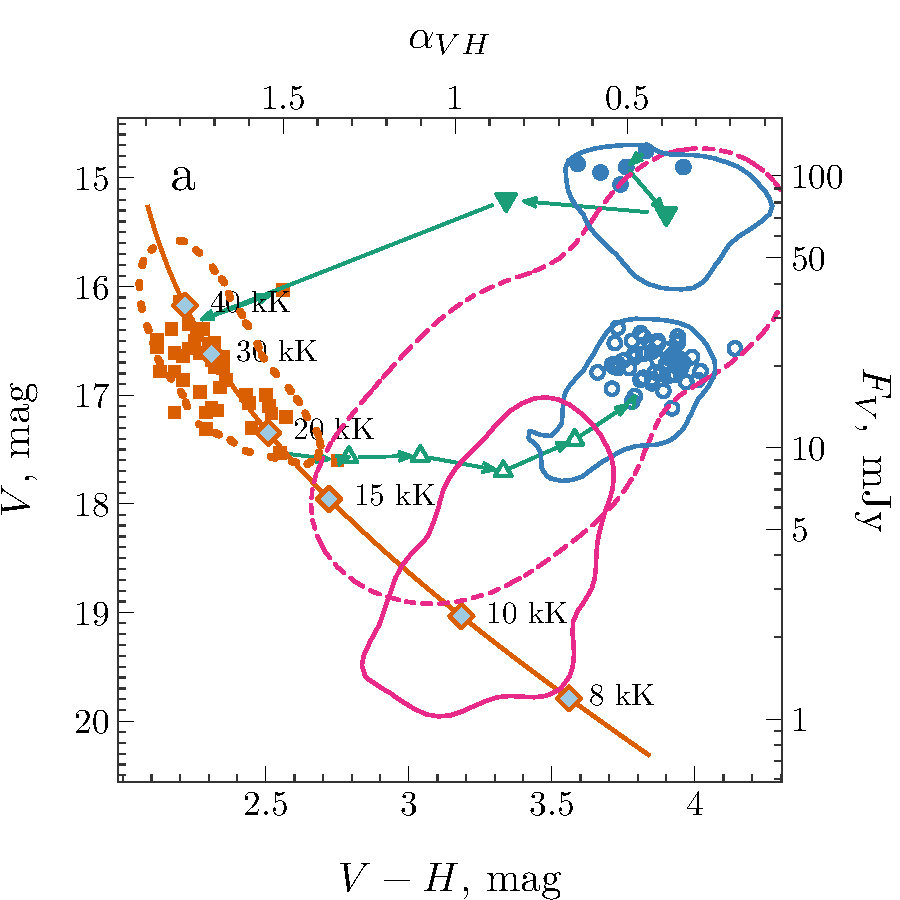
\includegraphics[keepaspectratio, width = 1\linewidth]{images/CMD_Contour_04.pdf}
    \caption{
        An example of \gls{CMD} plotted for \GX. 
        Different colours and symbols encode spectral states, with blue circles corresponding to the hard states, orange squares -- to the soft state, green triangles -- to the state transitions.
        90\% density contours for each state are computed using data from five outbursts observed in 2002--2010 period \citep{Buxton2012}.
        Solid blue contours correspond to the rising and decaying hard states, dotted orange -- to the soft state, dashed pink -- to the rising (from quiescent) phase, solid pink -- to the decaying phase.
        Solid orange line depicts blackbody model with fixed normalization and variable temperature.
        From \paperV.
    }
    \label{fig:bh-gx-colors}
\end{figure}


\subsection{Timing properties}
All accreting binary systems inherently demonstrate light curve variability on different timescales, and \glspl{BHXRB} are no exception.
Observed aperiodic and quasi-periodic variability profiles depend on the accretion state of the source, and change dramatically when a state transition occurs.


The \glspl{QPO} can be categorized into several types based on the centroid frequency $\nu_\mrm{c}$, relative width $\Delta\nu_\mrm{FWHM}/\nu_\mrm{c}$ (or its inverse value, quality $Q$), amplitude, and the shape of background (broadband) noise.
Low-frequency oscillations ($1-30$~Hz) are subdivided into three types: A, B, C \citep[][ also see Fig.~\ref{fig:bh-qpos}]{Casella2004}.
On rare occasions, \glspl{HFQPO} are also observed in the $40-450$~Hz range \citep{Belloni2012}.

\begin{figure}
    \centering
    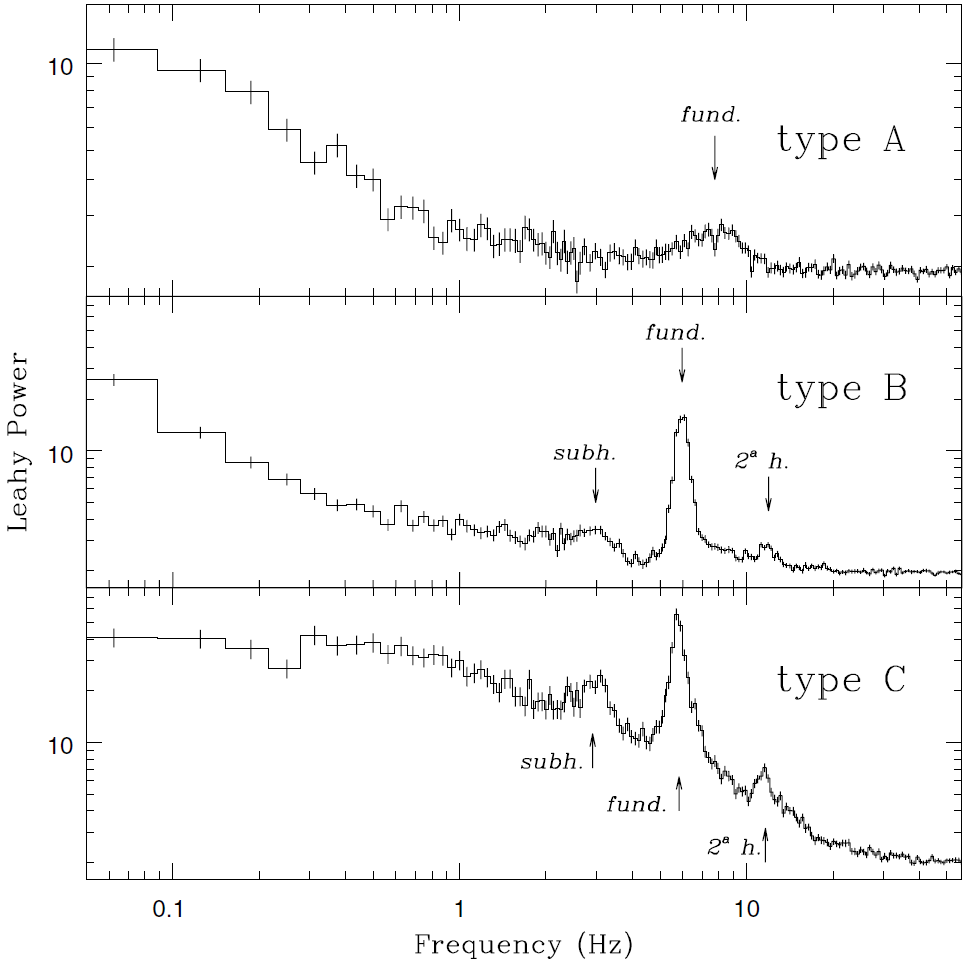
\includegraphics[keepaspectratio, width = 1\linewidth]{images/qpos.png}
    \caption{
        Examples of type A, B, and C \glspl{QPO} observed in \XTEJqpo.
        The Poisson noise is not subtracted and the \glspl{PSD} are normalized using Leahy normalization \citep{Leahy1983}.
        Adopted from \citet{Casella2004} (see their fig.~2).
    }
    \label{fig:bh-qpos}
\end{figure}


Although \glspl{QPO} have been detected in multiple sources, their nature is still debated.
Type-A \glspl{QPO}, present in the soft state after the hard-to-soft state transition, exhibit small amplitudes and large relative widths (small $Q$), which suggests they may originate from a disc instability.
Type-Bs are much more prominent and narrower, sometimes showing harmonic and subharmonic \citep{Casella2004}.
These \glspl{QPO} are observed to rapidly appear/disappear after then end of the hard state \citep{Motta2016}, which can be associated with the contribution of the relativistic jet \citep{Fender2009, Homan2020}.
Type-C \glspl{QPO} are mostly present in the hard state, but can be observed throughout the outburst \citep{Motta2016}.
They usually have high amplitude and one or more harmonics, while the centroid frequency can vary dramatically \citep{Motta2015}.
The \glspl{HFQPO} are only found at high fluxes in the soft-intermediate and high soft states \citep{Belloni2012}, yet it is still unclear whether it is a selection effect \citep{Motta2016, Ingram2019}.
\Glspl{HFQPO} can have one or two peaks (which can be spurious owing to the data processing methods, \citealt{Motta2016}), energy-dependent amplitude, and quality factors in the range of [5; 30] \citep{Ingram2019}.


\glspl{QPO} were detected in a wide range of energies, down to infrared \citep{Kalamkar2016}.
\glspl{QPO} are associated with different emitting components present in the \glspl{BHXRB}, and as the contribution of each component to the observed emission changes with wavelength, so do the \glspl{QPO}.
This can be seen in the \gls{CCF} of light curves obtained for two different energy ranges (e.g., optical and X-rays).
The \gls{CCF} highlights common variability patterns between two light curves, their correlation and potential offset in time.
Multiple signals observed in the \gls{CCF} are a signature of more than one component producing emission in both energy ranges.
The shape of each individual signal is a strong predictor of the emitting (or reprocessing) mechanism responsible for the short-term variability \citep[see, e.g, ][]{Malzac2004,Gandhi2008,Veledina2015,Omama2021}.
Thus, the \gls{CCF} analysis is an irreplaceable tool for decoupling non-thermal and disc components, especially during the hard state of outbursts.



On much longer time scales \glspl{BHXRB} can exhibit superhumps -- optical modulations originally observed in the superoutbursts of some dwarf novae \citep{Vogt1974,Warner1975,Osaki1996}.
Superhumps are believed to be caused by the 3:1 resonance within the accretion disc \citep{Whitehurst1991}.
The disc becomes eccentric and starts to slowly precess, resulting in a beat period that is a few per cent longer than the orbital (if the precession is prograde, otherwise the beat period is smaller than the orbital; \citealt{Donoghue1996, Zurita2002}).
Superhumps arise in systems with $q \lesssim 0.33$ and can be observed at any inclination.

Superhumps can be observed in both hard and soft states of \glspl{BHXRB}.
\glspl{BHXRB} may exhibit only superhump modulations and no orbital variability, so independent measurement of the orbital period are required (for instance, using spectroscopic observations of the secondary star during quiescence) to reliably identify observed variability as superhumps.
Some notable binaries exhibiting superhumps are \NMus\ \citep{Bailyn1992}, \XTEJxi\ \citep{Zurita2002}, \GX\ \paperVI, and \MAXI\ \citep{Torres2019}.


Optical modulations observed in \MAXI\ during the hard \citep{Patterson2018} and soft states \citep[\gls{AAVSO} data; \paperIV;][]{Kafka2020} have periods a few percent longer than the orbital period and are attributed to superhumps \citep{Torres2019}.
The magnitude of these modulations reaches $V \sim 0.4$~mag \citep{Patterson2018}.
However, polarimetric observations of \MAXI\ revealed no statistically significant variability in the soft state data \paperIVp, which were obtained quasi-simultaneously with the \gls{AAVSO} data showing $V \sim 0.1$~mag photometric superhump variability.
The absence of polarization modulations suggests that either the magnitude of these modulations is below the instrument detection limit, or that the source of photometric modulations produces unpolarized radiation and therefore does not contribute to the observed polarization.


\subsection{Polarization properties}
In recent years \gls{ONIR} polarimetry of \glspl{BHXRB} became an important tool for studying the properties of accreting black holes.
Unlike spectral and timing methods, measuring polarization of radiation provides information about orientation of the emitting/scattering components.
Some \glspl{BHXRB} exhibit small, but statistically significant intrinsic polarization in the active phase (\paperII; \citealt{Russell2018}; \paperIII), which can help understanding the source of the emission in the outburst.

There are two ways to produce polarized emission: either directly emitting polarized radiation, e.g., via synchrotron mechanism, or by scattering radiation by a non-spherical medium.
The first scenario requires strong ordered magnetic field, and the resulting polarized spectrum is expected to be non-thermal.
In the second scenario, the spectral shape of the polarized emission depends on the spectral shape of the source emission and on the scattering mechanism (its wavelength dependence and inelasticity).

From geometrical perspective, there is a single symmetry axis, the disc axis, which determines the polarization angle of emission.
The disc warp or presence of accretion winds can, however, affect the \gls{PA}.
It is possible to produce \gls{PA} parallel to the disc axis (sometimes believed to be also jet axis) by scattering in the slow accretion winds \paperIIp\ and in the mildly relativistic polar outflows \citep{Beloborodov1998,Beloborodov1999}, or emitting from the optically thin electron-scattering dominated non-spherical envelope.
The perpendicular configuration can be achieved in the optically thick envelope \citep[e.g.,][]{Sobolev1949,Sobolev1963}.
However, the polarization angle can be rotated by 90$^\circ$ at some viewing angles owing to the impact of absorption opacity \citep[Nagirner effect,][]{Nagirner1962}.
Thus, the intrinsic polarization parallel to the disc axis is the most likely to be observed.



\section{The origin of the non-thermal \glsentrytext{ONIR} emission}
\begin{figure}
    \centering
    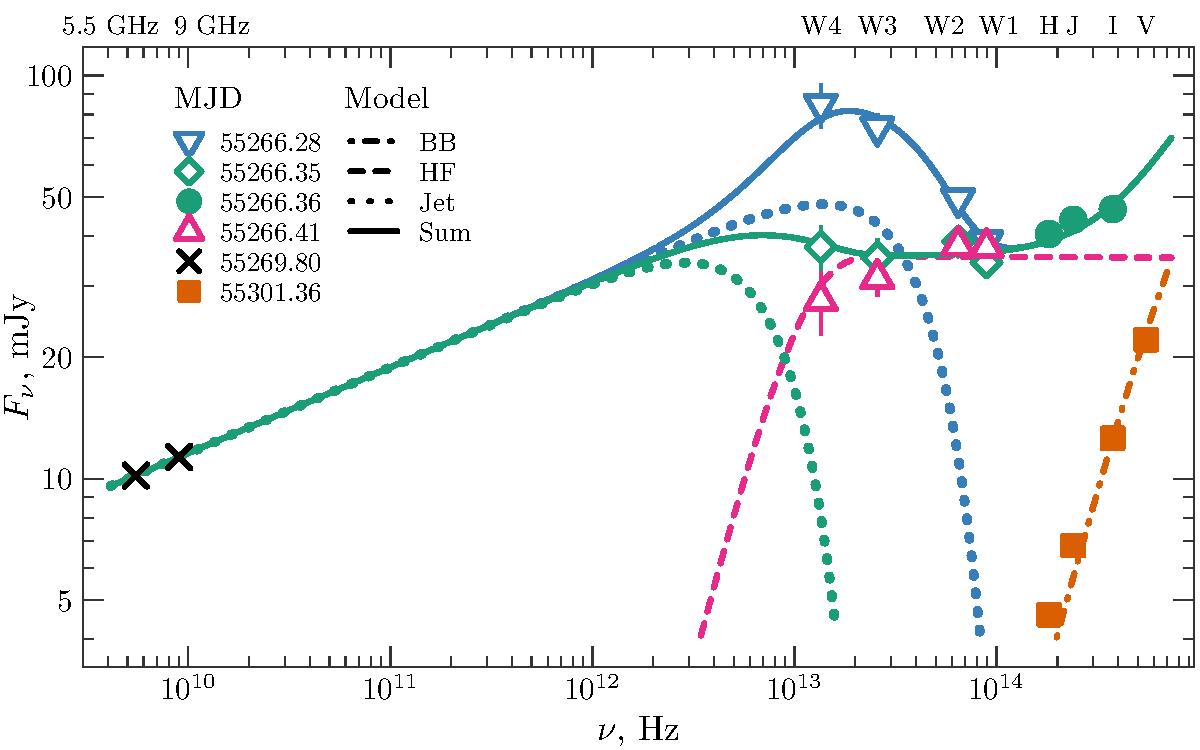
\includegraphics[keepaspectratio, width = 1\linewidth]{images/spec_dec_1.pdf}
    \caption{
        Broadband spectra of \GX\ using the radio \gls{ATCA}, \gls{midIR} \gls{WISE}, and \gls{ONIR} \gls{SMARTS} data.
        The figure shows four distinct spectral shapes for the source.
        The lines show different model components: the dot-dashed orange line indicates the blackbody component, the dashed pink line shows the hot flow component, the dotted lines correspond to the jet model with different cutoff frequencies, and the solid lines give the sum of the three (blackbody + hot flow+ jet) components.
        From \paperV.
    }
    \label{fig:gx_spec_dec}
\end{figure}

One of the distinctive features of the \gls{ONIR} spectra of \glspl{LMXB} is the `excess' above the disc emission observed in many systems during the hard state \citep{Hynes2000, Jain2001,Buxton2004, Kalemci2013}.
The excess component demonstrates spectra that are usually softer than the spectra of the underlying blackbody emission from the thin accretion disc \citep{Shakura1973}.
The emergence of this component (or components) produces flares, which are characteristic to \gls{ONIR} region, and appear during both rising and decaying hard states.

The complex \gls{ONIR} hard state spectra were initially modelled with the irradiated accretion disc, which reprocesses a portion of the X-ray radiation from the central machine and thus modifies its emitted spectrum \citep[e.g., \XTEJxviii,][]{Gierlinski2009}.
This model, however, requires a tight correlation between X-ray and optical emission and their timing properties \citep{VanParadijs1994}, violation of which is a strong indicator of another component contributing to the \gls{ONIR} emission.

Another component capable of emitting non-thermal radiation in the \gls{ONIR} region is jet.
The standard jet model \citep{Blandford1979} predicts that the jet produces partially absorbed hard spectrum ($F\propto \nu^\alpha$ where $\alpha = 5/2$) at low energies and optically thin soft ($\alpha = -(p-1)/2$ for the case of the simple power-law electron distribution as a function of Lorenz factor $\gamma$, $\mrm{d}n/\mrm{d}\gamma \propto \gamma ^ {-p}$, see \citealt{RadiationProcesses}) spectrum at higher energies.
The synchrotron break frequency, at which the jet spectrum changes its slope, is inversely proportional to the inner disc radius \citep{Heinz2003}, which is subject to change throughout the outburst.
Moreover, the jet is usually present in the hard state, but it is quenched in the disc-dominated soft state \citep{Corbel2002}, which explains the absence of the non-thermal excess in the soft spectra of \glspl{LMXB} if jet is responsible for it.
The jet contribution to the \gls{ONIR} region can be also predicted based on the spectral slope $\alpha$ ($F\sim \nu^\alpha$) observed in the radio, as low-frequency emission is dominated by the jet.
In \ivU\ \citep{Kalemci2005} and \MAXIJxviii\ \citep{Russell2013} the \gls{ONIR} flares are attributed to the evolution of the jet.


Non-thermal radiation can be also produced by the hot accretion flow.
Its spectra have two break frequencies between partially self-absorbed ($\alpha = 5/2$), fully absorbed (with $\alpha = (5\theta + \beta(2p + 3) -2p-8)/(\beta(p+2) + 2\theta)$, where magnetic field $B \propto R^{-\beta}$ and optical depth $\tau \propto R^{-\theta}$) and Comptonized parts \citep[see, e.g., ][]{Veledina2013, Poutanen2014a}.
The low-frequency break is determined by the extent of the accretion flow and evolves with time.
The outer parts of the hot flow may collapse or recover during state transitions, which affects the break frequency and overall shape of the produced spectrum.
The \XTEJxv\ \citep{Poutanen2014} and \SwiftJxvii\ \citep{Kajava2016} are examples of systems, in which accretion flows make significant contribution to the observed \gls{ONIR} hard state spectra, while the jet is highly unlikely to be responsible for the hard state \gls{ONIR} excess.


The origin of the non-thermal component in most systems is still debated \citep{Uttley2014, Poutanen2014a}.
Both optically thin jet and hot flow can manifest themselves in \gls{ONIR} in a somewhat similar manner, making it difficult to distinguish these two mechanisms based solely on \gls{ONIR} photometry.
\GX\ is a curious example of a \gls{LMXB}, in which \gls{midIR} and \gls{ONIR} radiation is a product of a complex interplay of jet, hot accretion flow and accretion disc.
In the hard state, \GX\ shows nearly flat de-reddened disc-subtracted \gls{ONIR} spectrum, which preserves its shape during state transitions \paperVp.
The spectral slope and luminosity of the red component rule out the jet as the primary source of the \gls{ONIR} non-thermal emission, as the extrapolated from the radio data jet spectrum \citep{Blandford1979} is inconsistent with the \gls{ONIR} data.
The absence of breaks in the non-thermal component spectra suggests that the excessive emission can be produced by the accretion flow if it does not fully collapse during state transitions, but rather transforms into a hot corona atop the disc.
As a result, the observed non-thermal emission originates from the fully absorbed part of the accretion flow spectrum, which favours moderate spectral slopes $\alpha \in [-0.5;0.5]$ \citep{Poutanen2014a}.
At the same time, the \gls{midIR} region is dominated by a rapidly varying component, which spectrum changes from nearly flat (similar to that of the accretion flow present in \gls{ONIR}) to soft with a cutoff in the \gls{midIR}.
The \gls{midIR} spectra correlate with the spectral slopes observed in radio -- a signature of the jet dominating the frequency range from radio up to \gls{midIR}.
A fit to the quasi-simultaneous broad band radio to optical spectra of \GX\ is shown in Fig.~\ref{fig:gx_spec_dec}.
The soft state data are well described by a single blackbody curve, while the hard state data are fit with a combination of three components, one of which (jet) changes its flux by a factor of $\sim 4$ on the timescale of hours.
A sharp cutoff of the jet spectrum in the \gls{midIR} results in little to no contribution to the \gls{ONIR} fluxes, which are well-described by a combination of disc blackbody and hot flow synchrotron emission.
The three-component interpretation is also in agreement with the complex \glspl{QPO} observed in \GX.
Its \gls{CCF} is wavelength-dependent \citep{Gandhi2010,Gandhi2011}, and is best explained if the \gls{ONIR} emission is a combination of synchrotron emission from the accretion flow and reprocessed radiation \citep{Veledina2011}.


The case of \GX\ shows that studying spectral and timing properties may be insufficient to reliably determine the nature of the non-thermal component in an \gls{LMXB}, trace the complex interplay of different emitting components and their evolution throughout the outbursts.
Polarization (or lack thereof) of an \gls{LMXB}, however, can provide a unique insight into the geometrical properties of the source and the structure of its magnetic field.
The changes in the intrinsic polarization (both degree and angle) during the state transitions observed in systems like \VCYG\ and \MAXI\ shed more light on the nature of the non-thermal components in these sources and help identify the primary emitting mechanism responsible for the \gls{ONIR} flares.
Thus, polarimetry has potential to augment existing techniques of \gls{LMXB} data analysis, allowing to draw a more detailed picture of the accretion processes in the vicinity of black holes.

% {\bf Plan}

% \begin{itemize}
%     +\item Accretion in binary systems (briefly mention HMXBs/LMXBs, Roche lobe, ideal for accretion studies in OIR)
%     +\item Outburst cycle: quiescent for decades, outburst on weeks-months timescales
%     +\item Main components (disc, jet, hot flow, winds)
%     +\item Contribution of different components can be probed by (i) broadband spectral shape and its evolution (colours), (ii) timing analysis (CCFs, QPOs and superhumps) and (iii) polarization
%     +\item Radiation at different wavelengths: radio from jet,  different components contribute 
%     +\item Detailed description of the first two possibilities - what can be probed, why and how (from our papers)
%     +\item Polarization as an emerging powerful tool to distinguish between components. Brief description which broadband polarization signatures can be expected from jet/disc/wind/hot flow (again, from our papers)
% \end{itemize}

